%%%%%%%% ICML 2021 EXAMPLE LATEX SUBMISSION FILE %%%%%%%%%%%%%%%%%

\documentclass{article}

% Recommended, but optional, packages for figures and better typesetting:
\usepackage{microtype}
\usepackage{graphicx}
\usepackage{subfigure}
\usepackage{booktabs} % for professional tables
\usepackage{amsmath}

% hyperref makes hyperlinks in the resulting PDF.
% If your build breaks (sometimes temporarily if a hyperlink spans a page)
% please comment out the following usepackage line and replace
% \usepackage{icml2021} with \usepackage[nohyperref]{icml2021} above.
\usepackage{hyperref}

% Attempt to make hyperref and algorithmic work together better:
\newcommand{\theHalgorithm}{\arabic{algorithm}}

% Use the following line for the initial blind version submitted for review:
%\usepackage{icml2021}

% If accepted, instead use the following line for the camera-ready submission:
\usepackage[accepted]{icml2021}

% The \icmltitle you define below is probably too long as a header.
% Therefore, a short form for the running title is supplied here:
\icmltitlerunning{Deep Supervision and Skip Connections in FCNs}

\begin{document}

\twocolumn[
\icmltitle{Understanding the Interaction Between Deep Supervision \\
           and Skip Connections in Fully Convolutional Networks}

% It is OKAY to include author information, even for blind
% submissions: the style file will automatically remove it for you
% unless you've provided the [accepted] option to the icml2021
% package.

\icmlsetsymbol{equal}{*}

\begin{icmlauthorlist}
\icmlauthor{João Vítor de Carvalho Silva}{ufmg}
\icmlauthor{Lucas de Oliveira Ferreira}{ufmg,abc}
\icmlauthor{Third Author}{abc}
\end{icmlauthorlist}

\icmlaffiliation{ufmg}{Universidade Federal de Minas Gerais, Belo Horizonte, Brazil}
\icmlaffiliation{abc}{ABC Institute, Rupert-Karls-University Heidelberg, Heidelberg, Germany}

\icmlcorrespondingauthor{João Vítor de Carvalho Silva}{lncs@springer.com}

% You may provide any keywords that you
% find helpful for describing your paper; these are used to populate
% the "keywords" metadata in the PDF but will not be shown in the document
\icmlkeywords{Auxiliary heads, Deep supervision, Image segmentation, Skip connections, Fully convolutional networks}

\vskip 0.3in
]

% this must go after the closing bracket ] following \twocolumn[ ...

\printAffiliationsAndNotice{}  % leave blank if no need to mention equal contribution

\begin{abstract}
Deep supervision through auxiliary exits is a well-known technique for improving
gradient flow in deep networks, but its effect on Fully Convolutional Networks
(FCNs) for semantic segmentation, and in particular its interaction with skip
connections, remains poorly understood. In this work we attach auxiliary
cross-entropy heads to the intermediate score maps of the classic FCN-32s,
FCN-16s and FCN-8s decoders, distinguishing exits placed \emph{before} any skip
fusion (s32, at the bottleneck) from exits placed \emph{after} the first fusion
(s16). Through a systematic study on the Semantic Boundaries Dataset (SBD),
covering auxiliary-weight sweeps, multiple simultaneous exits, skip-connection
removal, and alternative resolution-matching strategies, we show that deep
supervision is not universally beneficial: where the exit is placed matters more
than its weight. The post-fusion s16 exit consistently improves over the
baseline, whereas the pre-fusion s32 exit degrades every model that has skip
connections. Removing the skip connections increases the relative gain of the
auxiliary exit, and supervising at the native low resolution by downsampling the
label outperforms upscaling the prediction with bilinear interpolation or a
learnable deconvolution. These results, which transfer to fine-tuning on PASCAL
VOC 2011, reveal a strong interaction between auxiliary supervision and skip
connections and offer practical guidance on how deep supervision should be
applied to FCN-style architectures.
\end{abstract}

\section{Introduction}

    \subsection{Semantic Segmentation and FCNs}

    Image segmentation is used in many important tasks, such as in healthcare for detecting tumors, organs, or blood vessels in medical imaging; in autonomous driving to help self-driving cars identify lane markings, road signs, obstacles, and pedestrians; and in satellite imagery to analyze land use, urban growth, and agricultural zones. It works by classifying each pixel of an image into a class in order to segment the objects.

    The Fully Convolutional Network (FCN) \cite{ref_fcn} is a well-known architecture for image segmentation explored by [cite original paper]. It works similarly to an encoder-decoder architecture, but it adds skip connections to recover spatial data lost in the feature-extraction process.

    \subsection{Deep Supervision}

    In this paper, we explore how auxiliary exits affect the performance of Fully Convolutional Networks for semantic segmentation, depending on certain criteria. Although deep supervision has proven effective for enhancing gradient flow, as GoogLeNet \cite{ref_googlenet} showed, its effect on FCNs remains unclear. Moreover, its use for image segmentation in fully convolutional networks is not a silver bullet and must be applied with care, as we show in this paper.

    \subsection{Gap}

    Although auxiliary heads have been widely studied, the literature has not yet explored how they interact with skip connections. Thus, taking advantage of the fact that, in the upsampling block, the depth of the feature maps equals the number of classes, we explore what happens if we force a map to behave as an exit. This is possible because, during the upsampling phase, the maps behave almost like a low-resolution segmentation.

    \subsection{Contributions}

    (1) Wide evaluation on FCN8, FCN16 and FCN32; (2) Ablation over the deep supervision locations; (3) Several auxiliary weights; (4) Removal of skip connections; (5) Auxiliary upsampling branches; (6) Analysis of the interaction between supervision and skip connections

    To better compare with the literature, we also follow the original FCN approach: we train the models on the SBD dataset and fine-tune the pre-trained FCN weights on the VOC 2011 samples.


\section{Related Work}

    \subsection{Fully Convolutional Networks}
    FCNs \cite{ref_fcn} replace the fully connected layers with convolutions and, during decoding, fuse features from earlier layers with the deepest layer through deconvolution and skip connections (residual sums). Like ResNet \cite{ref_resnet} and U-Net \cite{ref_unet}, the models are optimized using only the loss at the final output, so the skip connections provide a useful path for the gradients to propagate.

    The original FCN models have three variants that differ only in the decoding strategy, as Figure \ref{fig_fcns} shows, sharing the same VGG-16 encoder and classifier.

    FCN32 is the simplest of them, as it upsamples the stride-32 map with a single x32 transposed convolution, and it has no skip connections.

    FCN16 introduces a single skip connection. The stride-32 map is upsampled by a factor of x2 and fused with a skip connection at stride-16. Lastly, it performs an x16 upscale to produce the final segmentation at the original resolution.

    FCN8 extends the skip-connection idea and is more complex. At stride-32, it performs an x2 upscale and then fuses a stride-16 skip connection. It then performs another x2 upscale and adds a second skip connection, this time from a stride-8 score map. Finally, it applies an x8 upscale at stride-8 to recover the original image resolution.

    \begin{figure*}[t]
    \begin{center}
    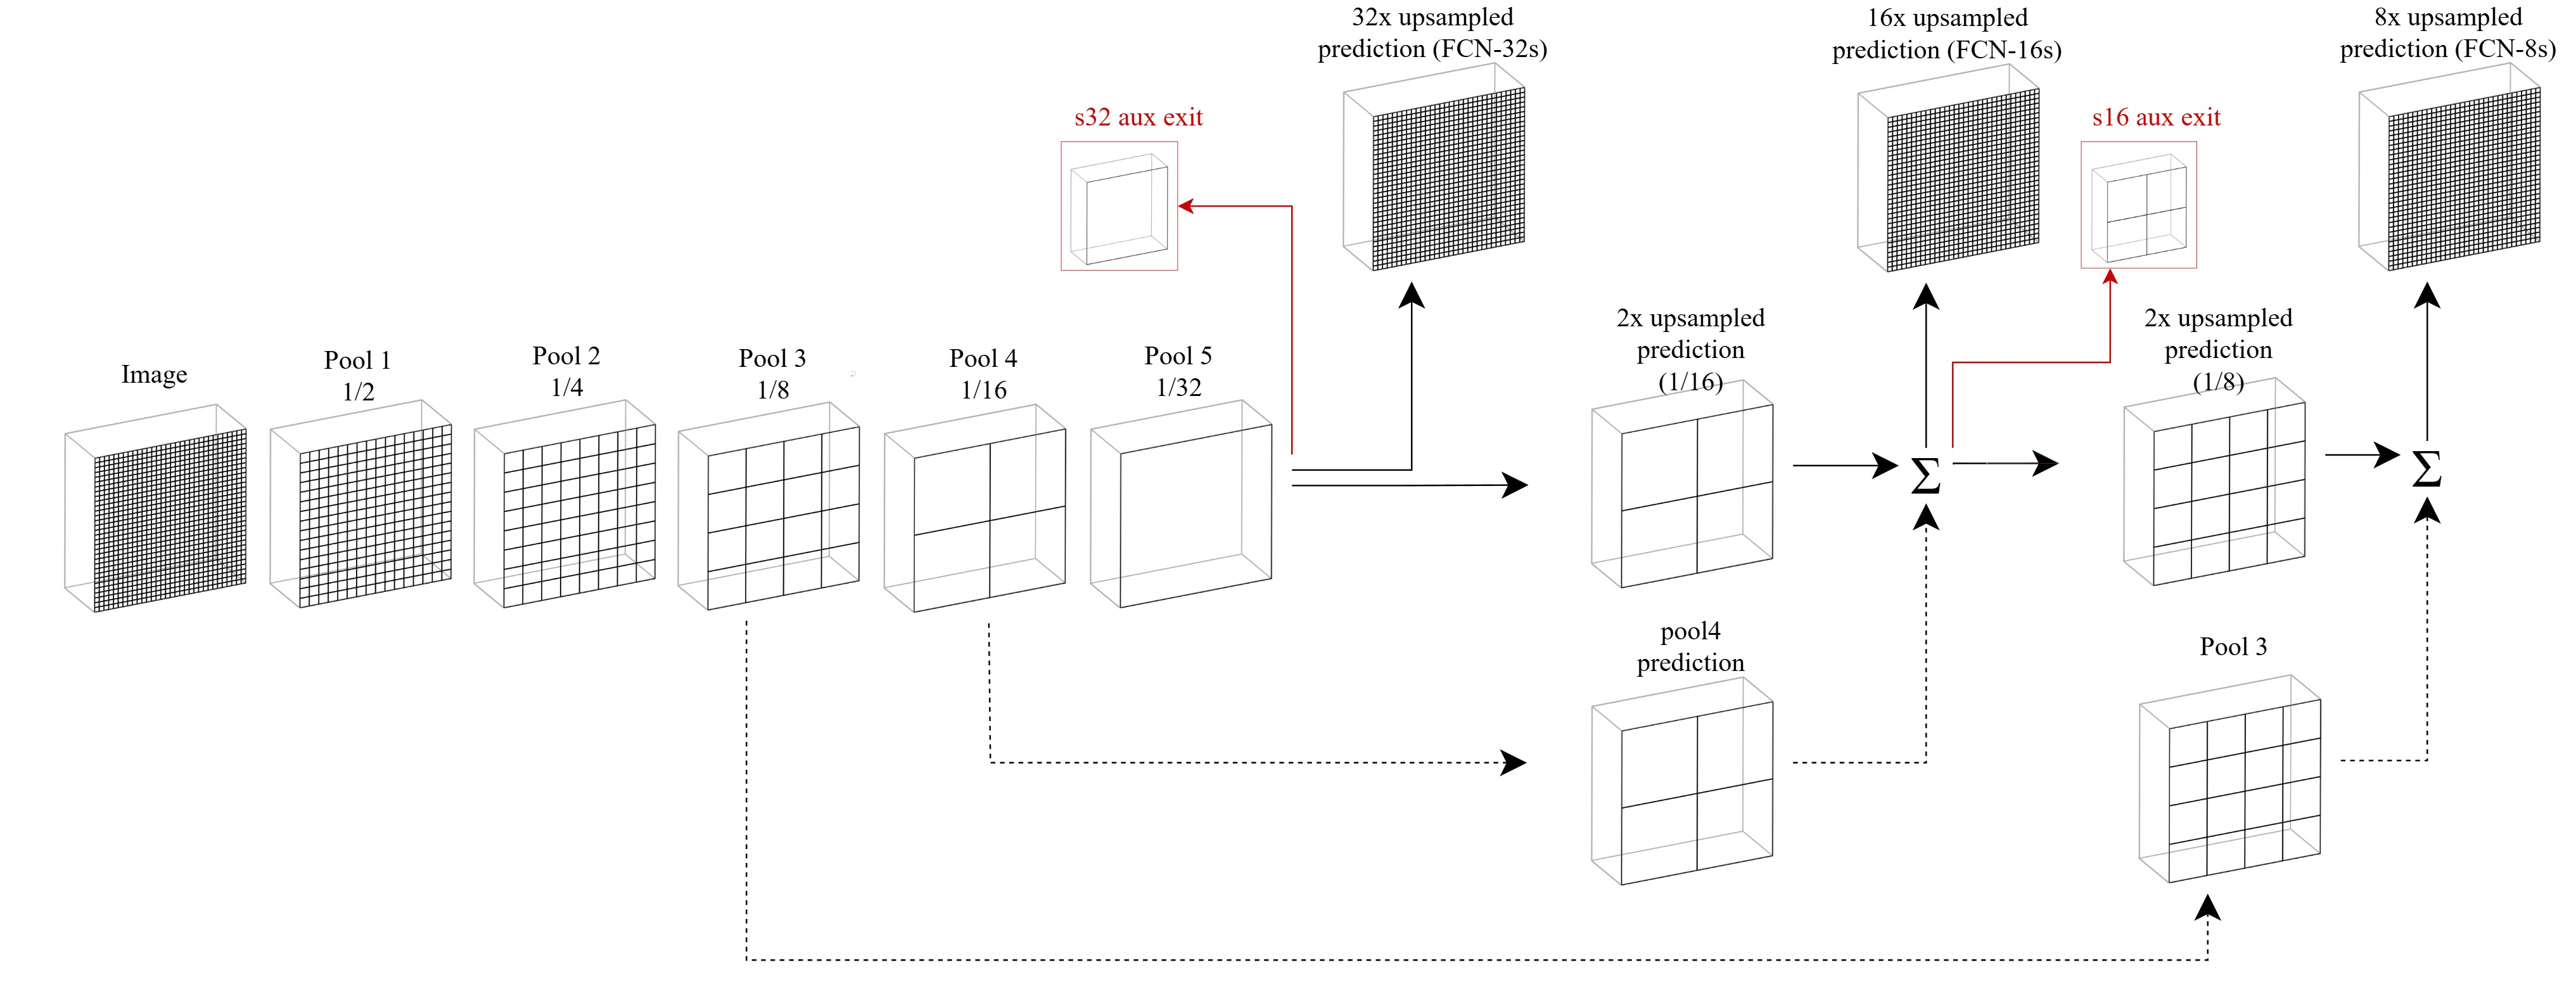
\includegraphics[width=\textwidth]{figures/fcn.jpg}
    \end{center}
    \caption{The auxiliary supervision can be attached either before the first skip connection (s32) or after the first skip fusion (s16). This distinction is central to our experimental analysis.}
    \label{fig_fcns}
    \end{figure*}

    Throughout this work, we refer to the intermediate prediction produced from the stride-32 feature map as "s32", and to the fused prediction after the first skip connection at stride 16 as "s16". So, s16 incorporates information from both the upsampled deep representation and the first skip connection, which makes it different from the original stride-16 features.


    \subsection{Deep supervision}
    The idea of influencing intermediary layers with auxiliary objectives dates back to multitask learning \cite{ref_multitask} when it comes to having multiple supervisions at the same task, and learning from hints, as \cite{ref_hints} initially explored. GoogLeNet \cite{ref_googlenet} uses discardable auxiliary classifiers, and DSN \cite{ref_dsn} showed that intermediate losses help combat vanishing gradients. For dense prediction, PSPNet \cite{ref_pspnet} adds a single auxiliary loss to an intermediate layer of a ResNet-based architecture, HED \cite{ref_hed} supervises side outputs, and UNet++ \cite{ref_unetpp} places auxiliary losses at several nodes. Unlike early-exiting architectures such as BranchyNet \cite{ref_branchynet}, our auxiliary exits are used only during training and are removed at inference time.



\section{Proposed Method}

    \subsection{FCN Architectures and Exit Points}

    We use the three classic FCN variants. The FCN-8s
    decoder computes:
    \begin{align}
    \texttt{score5} &= \mathrm{classifier}(\texttt{feat5}), \\
    \texttt{score4} &= \mathrm{score\_feat4}(\texttt{feat4}) + \mathrm{up}(\texttt{score5}), \\
    \texttt{score3} &= \mathrm{score\_feat3}(\texttt{feat3}) + \mathrm{up}(\texttt{score4}), \\
    h &= \mathrm{crop}(\mathrm{up}(\texttt{score3})),
    \end{align}
    where \texttt{score5} is the stride-32 bottleneck, \texttt{score4} the
    stride-16 map after the first fusion, \texttt{score3} the stride-8 map, and
    $h$ the final output at the original resolution. Here $\mathrm{up}(\cdot)$ is
    a transposed convolution (bilinearly
    initialized) and each sum is a skip connection. We define two auxiliary exit
    points: "s32", on \texttt{score5} (the bottleneck, \emph{before} any
    fusion), and "s16", on \texttt{score4} (\emph{after} the first fusion).
    FCN-16s has only the stride-16 fusion and FCN-32s has none (its output is
    \texttt{score5} upsampled directly).

    \subsection{Composite Auxiliary Loss}

    Each auxiliary exit produces intermediate score maps $P_a$ at its native
    resolution. The total loss sums the per-pixel cross-entropy
    ($\mathcal{L}_{\mathrm{CE}}$) of the main output with that of the active
    auxiliary exits, weighted by $\lambda_a$:
    \begin{equation}
    \mathcal{L}_{\mathrm{total}} = \mathcal{L}_{\mathrm{CE}}(Y, P_{\mathrm{main}})
    + \sum_{a} \lambda_a\, \mathcal{L}_{\mathrm{CE}}(Y_{\downarrow a}, P_a),
    \label{eq:loss}
    \end{equation}
    where $Y$ is the ground truth and $Y_{\downarrow a}$ is $Y$ \emph{downsampled}
    (nearest neighbor) to the resolution of $P_a$. Supervising at the native low
    resolution (downsampling the label) is our default approach, although we also tried training with an upscale branch; Sec.~\ref{sec:results}
    contrasts it with upscaling $P_a$.

    \subsection{Auxiliary Supervision Strategies}

    We compare two ways of matching the auxiliary prediction and the label:
    (i) \emph{downsampling} the label to the map resolution (default), and
    (ii) \emph{upscaling} the prediction to the original resolution, either with a
    learnable transposed convolution or with fixed bilinear interpolation.

    \subsection{Skip-Connection Removal}

    To test whether auxiliary exits and skip connections interact, we also train
    FCN8s with the skip connections removed (the output then flows only through
    the deep path), with and without the auxiliary exit.

    \subsection{Loss Weights}
    We sweep the auxiliary weight
\[
\lambda \in \{0.075,\ 0.1,\ 0.125,\ 0.2,\ 0.4\}.
\]

\section{Experiments}

    \subsection{Datasets and Setup}

    Following the original FCN protocol~\cite{ref_fcn}, we train on the Semantic
    Boundaries Dataset (SBD) and fine-tune the pre-trained weights on PASCAL VOC
    2011. [todo: Inserir split de treino e validação]. We train for 200 epochs with
    cross-entropy loss, [Adam optimizer], reporting
    mIoU and mean per-class pixel accuracy with validation at each epoch. Experiments ran on a single NVIDIA RTX 6000 (48\,GB) or a single NVIDIA Titan X (12\,GB) . [Especificar mais?]

    We report both the best mIoU and the mean mIoU over the last 20 epochs
    (``plateau''), the latter being more robust to spikes.

    \subsection{Configurations}
    We evaluate baselines (\texttt{1-exit}), single auxiliary exits at s32 and s16
    with various $\lambda$, a two-exit model (s16+s32), the no-skip ablation, and
    the upscaling variants (deconvolution and bilinear interpolation), followed by
    fine-tuning on VOC 2011.

    \subsection{RQ1: Does deep supervision improve FCN segmentation?}

    We first evaluate whether adding auxiliary supervision improves the
    baseline FCN architectures.

    \paragraph{Baselines}
    \begin{itemize}
        \item FCN32
        \item FCN16
        \item FCN8
    \end{itemize}

    \paragraph{Auxiliary supervision at stride 32}
    \begin{itemize}
        \item FCN32 + aux(s32)
        \item FCN16 + aux(s32)
        \item FCN8 + aux(s32)
    \end{itemize}

    \paragraph{Auxiliary supervision at stride 16 (FCN8)}
    \begin{itemize}
        \item $\lambda=0.075$
        \item $\lambda=0.10$
        \item $\lambda=0.125$
        \item $\lambda=0.20$
        \item $\lambda=0.40$
    \end{itemize}

    \paragraph{Multiple auxiliary heads} \hfill\newline
    FCN8 with simultaneous supervision at strides 32 and 16.

    \subsection{RQ2: Is the interaction with skip connections responsible for the observed behavior?}

    To investigate this hypothesis, we remove the skip connections from FCN8 and FCN16
    and repeat the experiments. For the auxiliary exits, we use $\lambda=0.10$.
    \begin{itemize}
        \item FCN8 (no skip)
        \item FCN8 (no skip + aux s16)
        \item FCN8 (no skip + aux s32)
        \item FCN16 (no skip)
        \item FCN16 (no skip + aux s32)
    \end{itemize}

    \subsection{RQ3: Is the degradation caused by supervising low-resolution feature maps?}

    To answer this question, we evaluate alternative supervision strategies.

    \begin{itemize}
        \item Direct supervision (baseline)
        \item Bilinear interpolation
        \item Learnable deconvolution branch
    \end{itemize}

    \subsection{RQ4: Does the improvement transfer to VOC?}

    The best-performing configuration obtained on SBD is fine-tuned on
    VOC 2011 and compared against the original FCN baselines.

    \begin{itemize}
        \item FCN8
        \item FCN8 + aux(s16) $\lambda=0.10$
        \item FCN16
    \end{itemize}


\section{Results}
\label{sec:results}

    \subsection{RQ1: Auxiliary Supervision Does Not Always Help}

        Table~\ref{tab:main} summarizes the SBD results. There is no general rule that
    auxiliary supervision improves FCNs: some configurations help and others hurt. The best configuration is \textbf{FCN-8s with an s16 exit and $\lambda=0.1$}. In contrast, the s32 exit degrades results in essentially every model with skip connections, and combining s16 and s32 (two exits) does not help.

        \begin{table}[t]
        \caption{SBD validation results. ``plateau'' is the mean mIoU over the last 20
        epochs. Models with a decoder degrade with the bottleneck exit (s32) and
        improve with the post-fusion exit (s16).}
        \label{tab:main}
        \vskip 0.15in
        \begin{center}
        \begin{small}
        \begin{tabular}{llcc}
        \toprule
        Model & Configuration & best mIoU & plateau mIoU \\
        \midrule
        FCN-32s & baseline & 0.312 & 0.298 \\
        FCN-32s & + aux s32 ($\lambda{=}0.4$) & 0.318 & 0.298 \\
        \midrule
        FCN-16s & baseline & 0.362 & 0.339 \\
        FCN-16s & + aux s32 ($\lambda{=}0.4$) & 0.327 & 0.306 \\
        \midrule
        FCN-8s & baseline & 0.359 & 0.341 \\
        FCN-8s & + aux s32 ($\lambda{=}0.1$) & 0.336 & 0.311 \\
        FCN-8s & + aux s16+s32 ($\lambda{=}0.4$) & 0.331 & 0.306 \\
        \textbf{FCN-8s} & \textbf{+ aux s16 ($\lambda{=}0.1$)} & \textbf{0.363} & \textbf{0.350} \\
        \bottomrule
        \end{tabular}
        \end{small}
        \end{center}
        \vskip -0.1in
        \end{table}

        \begin{figure}[t]\centering
      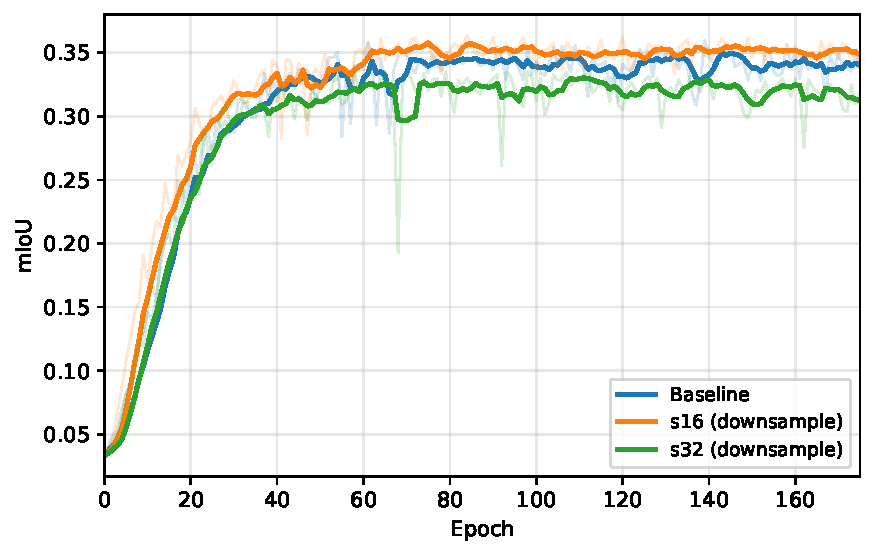
\includegraphics[width=\columnwidth]{figures/fig2_s16_vs_s32.pdf}
      \caption{FCN-8s on SBD: the post-fusion s16 exit improves over the baseline,
      while the pre-fusion s32 exit degrades it ($\lambda{=}0.1$).}
      \label{fig:s16s32}
    \end{figure}


    \paragraph{Position Matters More Than Weight:}
    When we vary $\lambda$ on the FCN-8s s16 exit, the weight changes the magnitude of the effect ($\lambda=0.1$ is best; large values such as $0.4$ wash the gain out), but the main factor is where the exit is placed: the gap between s16 and s32 is larger than any variation caused by $\lambda$.

    \paragraph{Why s32 Hurts and s16 Helps:}
    The difference appears to be related to what each tensor represents at the point of supervision. The s16 exit supervises score4 after fusion, a map that already combines score5 and deep spatial detail (feat4); it is naturally aligned with the segmentation objective, so reinforcing it helps optimization without interfering with the skip connections. The s32 exit supervises score5 before any fusion. On the main path, score5 is used through a learnable transposed convolution followed by a sum, giving the network freedom to shape its contribution. By supervising it directly, the auxiliary loss might remove that freedom and force it to be a good classifier, competing with the fine-grained objective of the main output for the shared weights.

    \subsection{RQ2: The No-Skip Experiment}
    \label{sec:noskip}
    To isolate the effect of the skip connections, we remove them from FCN-8s. As expected, the performance drops; however, the relative gain from the auxiliary exit increases: with skips, the s16 exit improves the plateau by $+0.008$ (0.341$\rightarrow$0.350), while without skips it improves by $+0.020$ (0.281$\rightarrow$0.301), as shown in Table~\ref{tab:res}. This suggests that when skip connections exist, they already provide an efficient path for information and gradient, with which auxiliary supervision may compete, and that when they are removed, the supervision partially compensates for their absence, supporting a strong interaction between the two mechanisms.
    \begin{figure}[t]\centering
      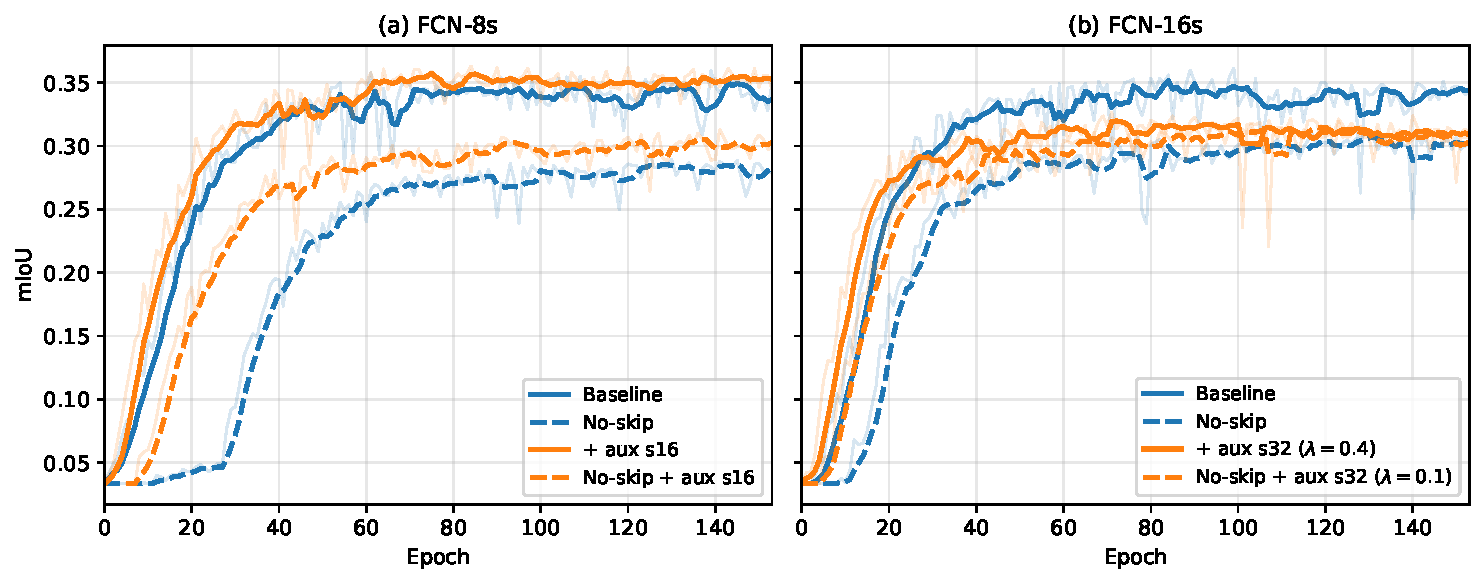
\includegraphics[width=\columnwidth]{figures/fig3_noskip.pdf}
      \caption{FCN-8s with and without skip connections: removing the skips lowers
      absolute mIoU, but the relative gain of the s16 exit grows ($+0.020$ vs.\
      $+0.008$ in plateau mIoU).}
      \label{fig:noskip}
    \end{figure}


    \paragraph{The Role of FCN-32s and the Architectural Gradient:}
    FCN-32s reinforces the argument: having no skip connections, its s32 exit nearly coincides with the final output, leaving no later fusion stage to be harmed (and indeed the effect is neutral): plateau 0.298 with and without the exit. The behavior across the FCNs indicates that the phenomenon is tied to the skip-connection fusions, not only to the depth of the auxiliary exit.
    \subsection{RQ3: Is downscaling the dataset the problem?}
    We also supervise the auxiliary exit at the original resolution by upscaling $P_a$ with (a) a learnable deconvolution and (b) bilinear interpolation, instead of downsampling the label. Neither helped; both hurt (Table~\ref{tab:res}). The learnable deconvolution was the worst (plateau 0.308, below the 0.341 baseline) and bilinear interpolation was intermediate. Comparing the three strategies at the same s16 exit, over a matched epoch window, yields the ordering \emph{label downsampling} $>$ \emph{baseline} $\approx$ \emph{interpolation} $>$ \emph{deconvolution}. We draw two conclusions: (i) inserting learnable layers between the auxiliary exit and the loss increases optimization complexity without adding information (deconvolution is worse than interpolation), and (ii) upscaling a coarse map to match the fine label is itself worse than matching at the native resolution, which provides a more reasonable target and supervises the representation directly.

    \begin{figure}[t]\centering
      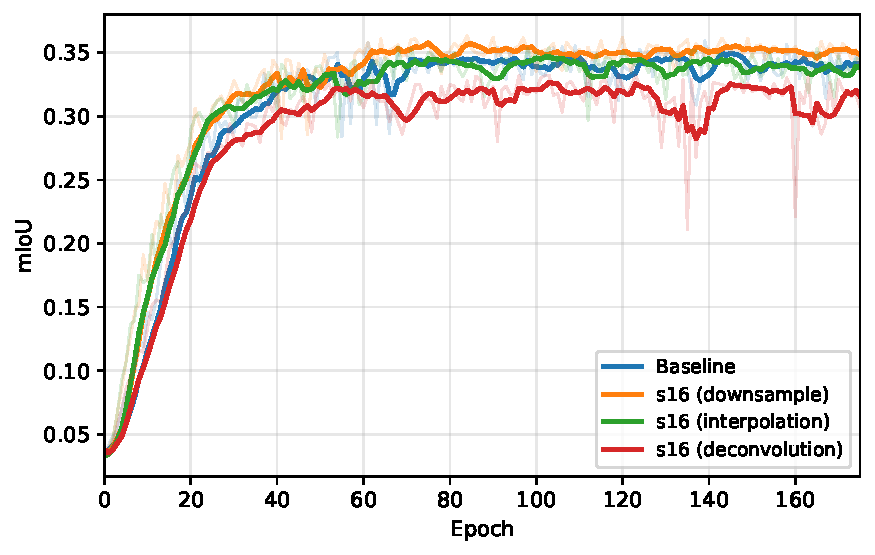
\includegraphics[width=\columnwidth]{figures/fig4_resolution.pdf}
      \caption{FCN-8s s16 exit: downsampling the label (native resolution) beats
      upscaling the prediction by bilinear interpolation or learnable
      deconvolution; the latter falls below the baseline.}
      \label{fig:resolution}
    \end{figure}


    \begin{table}[t]
    \caption{FCN-8s: skip-connection ablation and resolution-matching strategies
    (s16, $\lambda{=}0.1$). ``plateau'' is the mean mIoU over the last 20 epochs.}
    \label{tab:res}
    \vskip 0.15in
    \begin{center}
    \begin{small}
    \begin{tabular}{lcc}
    \toprule
    Configuration & best mIoU & plateau mIoU \\
    \midrule
    baseline (with skips) & 0.359 & 0.341 \\
    + aux s16 (label downsampling) & 0.363 & 0.350 \\
    + aux s16 (bilinear interpolation) & 0.356 & 0.337 \\
    + aux s16 (learnable deconvolution) & 0.333 & 0.309 \\
    \midrule
    no-skip baseline & 0.294 & 0.281 \\
    no-skip + aux s16 & 0.313 & 0.301 \\
    \bottomrule
    \end{tabular}
    \end{small}
    \end{center}
    \vskip -0.1in
    \end{table}

    \subsection{RQ4: Fine-tuning on the VOC 2011 dataset}
    We selected the most relevant models (FCN-32s, FCN-16s and FCN-8s baselines,
    and FCN-8s + s16 with $\lambda=0.1$) and fine-tuned them on the VOC 2011 dataset, using the weights trained on SBD. Although absolute values remain below those reported in the original work~\cite{ref_fcn}, the trend holds: the auxiliary-exit model keeps its advantage over the baseline [TODO: inserir números de VOC]. The effect is thus not specific to SBD.



\section{Conclusion}
In this paper, we investigated how auxiliary exits interact with the skip connections of the FCN architecture in the image segmentation task.
Supervising deep feature maps in a fully convolutional architecture can be beneficial, but it depends largely on where the auxiliary exit is placed. It is likely that supervising the feature maps before they are fused with skip connections can harm performance.
Although clearly understanding what happens inside a network is hard, we believe we have taken a step toward that goal.

%
\begin{thebibliography}{99}
\bibitem{ref_multitask}
Caruana, R.: Multitask learning. Machine Learning \textbf{28}, 41--75 (1997)

\bibitem{ref_hints}
Abu-Mostafa, Y.S.: Learning from hints in neural networks. Journal of
Complexity \textbf{6}(2), 192--198 (1990)

\bibitem{ref_googlenet}
Szegedy, C., Liu, W., Jia, Y., Sermanet, P., Reed, S., Anguelov, D., Erhan, D.,
Vanhoucke, V., Rabinovich, A.: Going deeper with convolutions. In: CVPR,
pp. 1--9 (2015)

\bibitem{ref_dsn}
Lee, C.-Y., Xie, S., Gallagher, P., Zhang, Z., Tu, Z.: Deeply-supervised nets.
In: AISTATS, pp. 562--570 (2015)

\bibitem{ref_fcn}
Long, J., Shelhamer, E., Darrell, T.: Fully convolutional networks for semantic
segmentation. In: CVPR, pp. 3431--3440 (2015)

\bibitem{ref_unet}
Ronneberger, O., Fischer, P., Brox, T.: U-Net: Convolutional networks for
biomedical image segmentation. In: MICCAI, pp. 234--241 (2015)

\bibitem{ref_resnet}
He, K., Zhang, X., Ren, S., Sun, J.: Deep residual learning for image
recognition. In: CVPR, pp. 770--778 (2016)

\bibitem{ref_pspnet}
Zhao, H., Shi, J., Qi, X., Wang, X., Jia, J.: Pyramid scene parsing network.
In: CVPR, pp. 2881--2890 (2017)

\bibitem{ref_hed}
Xie, S., Tu, Z.: Holistically-nested edge detection. In: ICCV,
pp. 1395--1403 (2015)

\bibitem{ref_unetpp}
Zhou, Z., Rahman Siddiquee, M.M., Tajbakhsh, N., Liang, J.: UNet++: A nested
U-Net architecture for medical image segmentation. In: DLMIA, pp. 3--11 (2018)

\bibitem{ref_branchynet}
Teerapittayanon, S., McDanel, B., Kung, H.T.: BranchyNet: Fast inference via
early exiting from deep neural networks. In: ICPR, pp. 2464--2469 (2016)
\end{thebibliography}

\end{document}
